\documentclass[ignorenonframetext,]{beamer}
\setbeamertemplate{caption}[numbered]
\setbeamertemplate{caption label separator}{: }
\setbeamercolor{caption name}{fg=normal text.fg}
\beamertemplatenavigationsymbolsempty
\usepackage{lmodern}
\usepackage{amssymb,amsmath}
\usepackage{ifxetex,ifluatex}
\usepackage{fixltx2e} % provides \textsubscript
\ifnum 0\ifxetex 1\fi\ifluatex 1\fi=0 % if pdftex
  \usepackage[T1]{fontenc}
  \usepackage[utf8]{inputenc}
\else % if luatex or xelatex
  \ifxetex
    \usepackage{mathspec}
  \else
    \usepackage{fontspec}
  \fi
  \defaultfontfeatures{Ligatures=TeX,Scale=MatchLowercase}
\fi
\usefonttheme{structurebold}
% use upquote if available, for straight quotes in verbatim environments
\IfFileExists{upquote.sty}{\usepackage{upquote}}{}
% use microtype if available
\IfFileExists{microtype.sty}{%
\usepackage{microtype}
\UseMicrotypeSet[protrusion]{basicmath} % disable protrusion for tt fonts
}{}
\newif\ifbibliography
\usepackage{color}
\usepackage{fancyvrb}
\newcommand{\VerbBar}{|}
\newcommand{\VERB}{\Verb[commandchars=\\\{\}]}
\DefineVerbatimEnvironment{Highlighting}{Verbatim}{commandchars=\\\{\}}
% Add ',fontsize=\small' for more characters per line
\usepackage{framed}
\definecolor{shadecolor}{RGB}{248,248,248}
\newenvironment{Shaded}{\begin{snugshade}}{\end{snugshade}}
\newcommand{\KeywordTok}[1]{\textcolor[rgb]{0.13,0.29,0.53}{\textbf{{#1}}}}
\newcommand{\DataTypeTok}[1]{\textcolor[rgb]{0.13,0.29,0.53}{{#1}}}
\newcommand{\DecValTok}[1]{\textcolor[rgb]{0.00,0.00,0.81}{{#1}}}
\newcommand{\BaseNTok}[1]{\textcolor[rgb]{0.00,0.00,0.81}{{#1}}}
\newcommand{\FloatTok}[1]{\textcolor[rgb]{0.00,0.00,0.81}{{#1}}}
\newcommand{\ConstantTok}[1]{\textcolor[rgb]{0.00,0.00,0.00}{{#1}}}
\newcommand{\CharTok}[1]{\textcolor[rgb]{0.31,0.60,0.02}{{#1}}}
\newcommand{\SpecialCharTok}[1]{\textcolor[rgb]{0.00,0.00,0.00}{{#1}}}
\newcommand{\StringTok}[1]{\textcolor[rgb]{0.31,0.60,0.02}{{#1}}}
\newcommand{\VerbatimStringTok}[1]{\textcolor[rgb]{0.31,0.60,0.02}{{#1}}}
\newcommand{\SpecialStringTok}[1]{\textcolor[rgb]{0.31,0.60,0.02}{{#1}}}
\newcommand{\ImportTok}[1]{{#1}}
\newcommand{\CommentTok}[1]{\textcolor[rgb]{0.56,0.35,0.01}{\textit{{#1}}}}
\newcommand{\DocumentationTok}[1]{\textcolor[rgb]{0.56,0.35,0.01}{\textbf{\textit{{#1}}}}}
\newcommand{\AnnotationTok}[1]{\textcolor[rgb]{0.56,0.35,0.01}{\textbf{\textit{{#1}}}}}
\newcommand{\CommentVarTok}[1]{\textcolor[rgb]{0.56,0.35,0.01}{\textbf{\textit{{#1}}}}}
\newcommand{\OtherTok}[1]{\textcolor[rgb]{0.56,0.35,0.01}{{#1}}}
\newcommand{\FunctionTok}[1]{\textcolor[rgb]{0.00,0.00,0.00}{{#1}}}
\newcommand{\VariableTok}[1]{\textcolor[rgb]{0.00,0.00,0.00}{{#1}}}
\newcommand{\ControlFlowTok}[1]{\textcolor[rgb]{0.13,0.29,0.53}{\textbf{{#1}}}}
\newcommand{\OperatorTok}[1]{\textcolor[rgb]{0.81,0.36,0.00}{\textbf{{#1}}}}
\newcommand{\BuiltInTok}[1]{{#1}}
\newcommand{\ExtensionTok}[1]{{#1}}
\newcommand{\PreprocessorTok}[1]{\textcolor[rgb]{0.56,0.35,0.01}{\textit{{#1}}}}
\newcommand{\AttributeTok}[1]{\textcolor[rgb]{0.77,0.63,0.00}{{#1}}}
\newcommand{\RegionMarkerTok}[1]{{#1}}
\newcommand{\InformationTok}[1]{\textcolor[rgb]{0.56,0.35,0.01}{\textbf{\textit{{#1}}}}}
\newcommand{\WarningTok}[1]{\textcolor[rgb]{0.56,0.35,0.01}{\textbf{\textit{{#1}}}}}
\newcommand{\AlertTok}[1]{\textcolor[rgb]{0.94,0.16,0.16}{{#1}}}
\newcommand{\ErrorTok}[1]{\textcolor[rgb]{0.64,0.00,0.00}{\textbf{{#1}}}}
\newcommand{\NormalTok}[1]{{#1}}
\usepackage{graphicx,grffile}
\makeatletter
\def\maxwidth{\ifdim\Gin@nat@width>\linewidth\linewidth\else\Gin@nat@width\fi}
\def\maxheight{\ifdim\Gin@nat@height>\textheight0.8\textheight\else\Gin@nat@height\fi}
\makeatother
% Scale images if necessary, so that they will not overflow the page
% margins by default, and it is still possible to overwrite the defaults
% using explicit options in \includegraphics[width, height, ...]{}
\setkeys{Gin}{width=\maxwidth,height=\maxheight,keepaspectratio}

% Prevent slide breaks in the middle of a paragraph:
\widowpenalties 1 10000
\raggedbottom

\AtBeginPart{
  \let\insertpartnumber\relax
  \let\partname\relax
  \frame{\partpage}
}
\AtBeginSection{
  \ifbibliography
  \else
    \let\insertsectionnumber\relax
    \let\sectionname\relax
    \frame{\sectionpage}
  \fi
}
\AtBeginSubsection{
  \let\insertsubsectionnumber\relax
  \let\subsectionname\relax
  \frame{\subsectionpage}
}

\setlength{\emergencystretch}{3em}  % prevent overfull lines
\providecommand{\tightlist}{%
  \setlength{\itemsep}{0pt}\setlength{\parskip}{0pt}}
\setcounter{secnumdepth}{0}
\definecolor{links}{HTML}{800080}
\hypersetup{colorlinks,linkcolor=,urlcolor=links}

\title{Web Data Collection with R}
\subtitle{JSON/API Case Study}
\author{Peter Meißner / 2016-02-29 -- 2016-03-04 / ECPR WSMT}
\date{}

\begin{document}
\frame{\titlepage}

\begin{frame}
\tableofcontents[hideallsubsections]
\end{frame}

\section{The old wikipedia pageviews API -
stats.grok.se}\label{the-old-wikipedia-pageviews-api---stats.grok.se}

\begin{frame}[fragile]{packages}

\begin{Shaded}
\begin{Highlighting}[]
\KeywordTok{library}\NormalTok{(rvest)}
\KeywordTok{library}\NormalTok{(jsonlite)}
\KeywordTok{library}\NormalTok{(lubridate)}
\KeywordTok{library}\NormalTok{(dplyr)}
\end{Highlighting}
\end{Shaded}

\url{http://stats.grok.se/}

\end{frame}

\begin{frame}[fragile]{A first try}

\begin{Shaded}
\begin{Highlighting}[]
\NormalTok{url  <-}\StringTok{ "http://stats.grok.se/json/en/latest90/Influenza"}
\NormalTok{json <-}\StringTok{ }\KeywordTok{html_text}\NormalTok{(}\KeywordTok{read_html}\NormalTok{(url)) }
\NormalTok{json}
\end{Highlighting}
\end{Shaded}

\begin{verbatim}
## [1] "{\"daily_views\": {\"2015-12-17\": 2100, \"2015-12-07\": 2424, \"2015-12-06\": 1728, \"2016-01-04\": 2580, \"2016-01-05\": 2431, \"2015-12-09\": 2704, \"2015-12-08\": 2490, \"2016-01-01\": 1247, \"2016-01-02\": 1260, \"2016-01-03\": 1517, \"2015-12-03\": 2421, \"2015-12-02\": 2446, \"2015-12-01\": 2587, \"2016-01-08\": 2002, \"2016-01-09\": 1418, \"2015-12-05\": 1374, \"2015-12-04\": 2037, \"2015-12-21\": 1684, \"2015-12-20\": 1220, \"2015-12-23\": 1256, \"2015-12-22\": 1553, \"2015-12-25\": 738, \"2015-12-24\": 1008, \"2015-12-27\": 1027, \"2015-12-26\": 862, \"2015-12-29\": 2647, \"2015-12-28\": 1340, \"2016-01-07\": 2163, \"2016-01-06\": 2426, \"2016-01-19\": 2778, \"2016-01-18\": 2347, \"2016-01-13\": 2651, \"2016-01-12\": 2560, \"2016-01-11\": 2505, \"2016-01-10\": 1767, \"2016-01-17\": 1626, \"2016-01-16\": 1439, \"2016-01-15\": 2282, \"2016-01-14\": 2515, \"2015-12-16\": 2351, \"2015-12-14\": 2196, \"2015-12-15\": 2200, \"2015-12-30\": 2212, \"2015-12-31\": 1604, \"2015-12-10\": 2398, \"2015-12-11\": 1855, \"2015-12-12\": 1355, \"2015-12-13\": 1656, \"2015-12-18\": 1880, \"2015-12-19\": 1163, \"2016-01-20\": 2886}, \"project\": \"en\", \"month\": \"latest90\", \"rank\": 3746, \"title\": \"Influenza\"}"
\end{verbatim}

\end{frame}

\begin{frame}[fragile]{A first try}

\begin{verbatim}
## {"daily_views": {"2015-12-17": 2100,
##   "2015-12-07": 2424,
##   "2015-12-06": 1728,
##   "2016-01-04": 2580,
##   "2016-01-05": 2431,
##   "2015-12-09": 2704,
##   "2015-12-08": 2490,
##   "2016-01-01": 1247,
##   "2016-01-02": 1260,
##   "2016-01-03": 1517,
##   "2015-12-03": 2421,
##   "2015-12-02": 2446,
##   "2015-12-01": 2587,
##  
## ...
\end{verbatim}

\end{frame}

\begin{frame}[fragile]{Getting JSON in}

\begin{Shaded}
\begin{Highlighting}[]
\NormalTok{data  <-}\StringTok{ }\KeywordTok{fromJSON}\NormalTok{(json)}
\NormalTok{date  <-}\StringTok{ }\KeywordTok{as.Date}\NormalTok{(}\KeywordTok{names}\NormalTok{(data$daily_views))}
\NormalTok{views <-}\StringTok{ }\KeywordTok{unlist}\NormalTok{(data$daily_views)}

\KeywordTok{plot}\NormalTok{( date, views,  }
      \DataTypeTok{ylim =} \KeywordTok{c}\NormalTok{(}\DecValTok{0}\NormalTok{, }\DecValTok{3000}\NormalTok{),}
      \DataTypeTok{type =} \StringTok{"h"}\NormalTok{, }
      \DataTypeTok{col  =} \StringTok{"#F54B1A90"}\NormalTok{,}
      \DataTypeTok{lwd=}\DecValTok{3}\NormalTok{, }
      \DataTypeTok{main=}\StringTok{"Influenca Page Views on Wikipedia (en)"}\NormalTok{)}

\KeywordTok{lines}\NormalTok{(}\KeywordTok{lowess}\NormalTok{(views ~}\StringTok{ }\NormalTok{date), }\DataTypeTok{col =} \StringTok{"#1B346C90"}\NormalTok{, }\DataTypeTok{lwd=}\DecValTok{5}\NormalTok{)}
\end{Highlighting}
\end{Shaded}

\end{frame}

\begin{frame}{Getting JSON in}

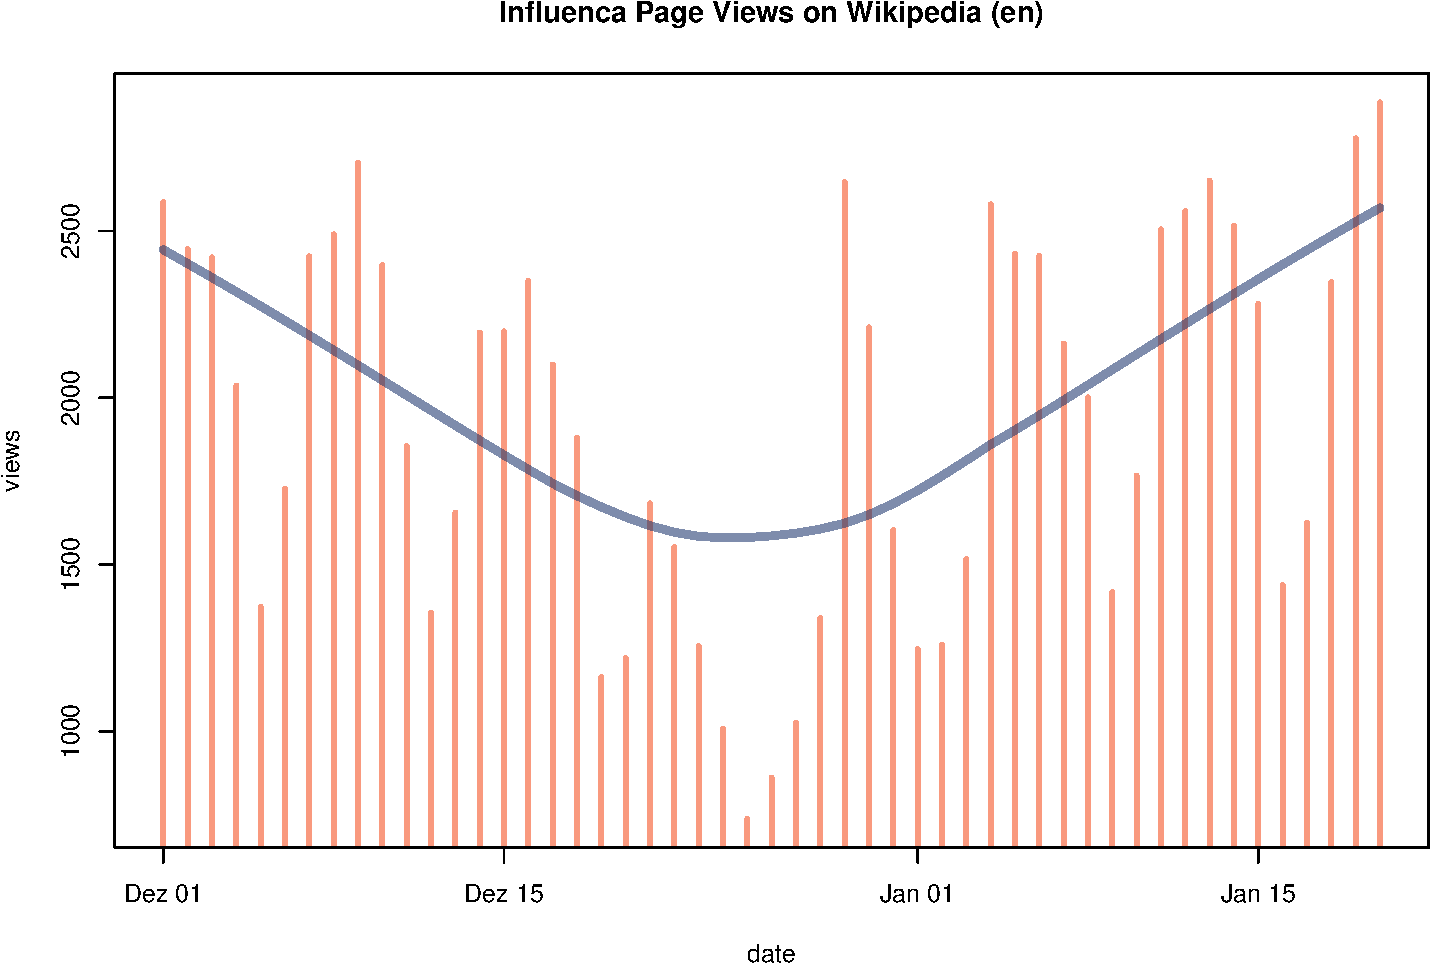
\includegraphics{json_case_files/figure-beamer/unnamed-chunk-5-1.pdf}

\end{frame}

\begin{frame}[fragile]{Getting serious}

\begin{Shaded}
\begin{Highlighting}[]
\NormalTok{url_pt1  <-}\StringTok{ "http://stats.grok.se/json/en/"}
\NormalTok{url_pt2  <-}\StringTok{ }
\StringTok{  }\KeywordTok{paste0}\NormalTok{(}
    \KeywordTok{rep}\NormalTok{(}\DecValTok{2014}\NormalTok{:}\DecValTok{2015}\NormalTok{, }\DataTypeTok{each=}\DecValTok{12}\NormalTok{),}
    \KeywordTok{str_pad}\NormalTok{(}\DecValTok{1}\NormalTok{:}\DecValTok{12}\NormalTok{, }\DataTypeTok{width=}\DecValTok{2}\NormalTok{, }\DataTypeTok{side=}\StringTok{"left"}\NormalTok{, }\StringTok{"0"}\NormalTok{)}
  \NormalTok{)}
\NormalTok{url_pt3  <-}\StringTok{ "/Influenza"}
\NormalTok{URL <-}\StringTok{ }\KeywordTok{paste0}\NormalTok{(url_pt1, url_pt2, url_pt3)}
\end{Highlighting}
\end{Shaded}

\end{frame}

\begin{frame}[fragile]{Getting serious}

\begin{Shaded}
\begin{Highlighting}[]
\CommentTok{# downloadig the data}
\NormalTok{JSON <-}\StringTok{ }\KeywordTok{list}\NormalTok{()}
\NormalTok{for( i in }\KeywordTok{seq_along}\NormalTok{(URL) )\{}
  \NormalTok{fname <-}\StringTok{ }\KeywordTok{basename}\NormalTok{(}\KeywordTok{dirname}\NormalTok{(URL[i]))}
  \NormalTok{if( !}\KeywordTok{file.exists}\NormalTok{(fname) )\{}
    \KeywordTok{download.file}\NormalTok{(URL[i], fname )}
    \KeywordTok{Sys.sleep}\NormalTok{(}\DecValTok{1}\NormalTok{)}
  \NormalTok{\}}
  \NormalTok{JSON[i] <-}\StringTok{ }\KeywordTok{readLines}\NormalTok{(fname, }\DataTypeTok{warn =} \OtherTok{FALSE}\NormalTok{)}
\NormalTok{\}}
\end{Highlighting}
\end{Shaded}

\end{frame}

\begin{frame}[fragile]{Getting serious}

\begin{Shaded}
\begin{Highlighting}[]
\CommentTok{# parsing the JSON}
\NormalTok{JSON_parsed <-}\StringTok{ }\KeywordTok{lapply}\NormalTok{(JSON, fromJSON)}

\NormalTok{json <-}\StringTok{ }\NormalTok{JSON_parsed[[}\DecValTok{1}\NormalTok{]]}

\NormalTok{date <-}\StringTok{ }
\StringTok{  }\NormalTok{json$daily_views %>%}\StringTok{ }
\StringTok{  }\KeywordTok{names}\NormalTok{() %>%}\StringTok{ }
\StringTok{  }\KeywordTok{ymd}\NormalTok{()}

\NormalTok{views <-}\StringTok{ }
\StringTok{  }\NormalTok{json$daily_views %>%}\StringTok{ }
\StringTok{  }\KeywordTok{unlist}\NormalTok{()}

\NormalTok{views[}\DecValTok{1}\NormalTok{:}\DecValTok{3}\NormalTok{]}
\end{Highlighting}
\end{Shaded}

\begin{verbatim}
## 2014-01-15 2014-01-14 2014-01-17 
##       6009       5951       5219
\end{verbatim}

\begin{Shaded}
\begin{Highlighting}[]
\NormalTok{date[}\DecValTok{1}\NormalTok{:}\DecValTok{3}\NormalTok{]}
\end{Highlighting}
\end{Shaded}

\begin{verbatim}
## [1] "2014-01-15 UTC" "2014-01-14 UTC" "2014-01-17 UTC"
\end{verbatim}

\end{frame}

\begin{frame}[fragile]{Getting serious}

\begin{Shaded}
\begin{Highlighting}[]
\CommentTok{# putting it in a function}
\NormalTok{page_views_to_df <-}\StringTok{ }\NormalTok{function(json)\{}
  \NormalTok{date  <-}\StringTok{ }\NormalTok{json$daily_views %>%}\StringTok{ }\KeywordTok{names}\NormalTok{() %>%}\StringTok{ }\KeywordTok{ymd}\NormalTok{()}
  \NormalTok{views <-}\StringTok{ }\NormalTok{json$daily_views %>%}\StringTok{ }\KeywordTok{unlist}\NormalTok{()}
  \NormalTok{df <-}\StringTok{ }\KeywordTok{data.frame}\NormalTok{(date, views)[!}\KeywordTok{is.na}\NormalTok{(date),]}
  \KeywordTok{rownames}\NormalTok{(df) <-}\StringTok{ }\OtherTok{NULL}
  \KeywordTok{return}\NormalTok{(df)}
\NormalTok{\}}
\end{Highlighting}
\end{Shaded}

\end{frame}

\begin{frame}[fragile]{Getting serious}

\begin{Shaded}
\begin{Highlighting}[]
\NormalTok{influenza15 <-}\StringTok{ }
\StringTok{  }\NormalTok{JSON_parsed %>%}\StringTok{ }
\StringTok{  }\KeywordTok{lapply}\NormalTok{(page_views_to_df) %>%}\StringTok{ }
\StringTok{  }\KeywordTok{do.call}\NormalTok{(rbind, .) }
\end{Highlighting}
\end{Shaded}

\begin{verbatim}
## Warning: 3 failed to parse.
\end{verbatim}

\begin{verbatim}
## Warning: 1 failed to parse.

## Warning: 1 failed to parse.

## Warning: 1 failed to parse.

## Warning: 1 failed to parse.
\end{verbatim}

\begin{verbatim}
## Warning: 3 failed to parse.
\end{verbatim}

\begin{verbatim}
## Warning: 1 failed to parse.

## Warning: 1 failed to parse.
\end{verbatim}

\end{frame}

\begin{frame}[fragile]{Getting serious}

\begin{Shaded}
\begin{Highlighting}[]
\KeywordTok{plot}\NormalTok{( influenza15$date, influenza15$views,  }
      \DataTypeTok{type =} \StringTok{"h"}\NormalTok{, }
      \DataTypeTok{col  =} \StringTok{"#F54B1A90"}\NormalTok{,}
      \DataTypeTok{lwd=}\DecValTok{1}\NormalTok{, }
      \DataTypeTok{main=}\StringTok{"Influenca Page Views on Wikipedia (en)"}\NormalTok{)}

\KeywordTok{lowess}\NormalTok{(influenza15$views ~}\StringTok{ }\NormalTok{influenza15$date, }\DataTypeTok{f=}\FloatTok{0.08}\NormalTok{) %>%}\StringTok{ }
\StringTok{  }\KeywordTok{lines}\NormalTok{(}\DataTypeTok{col =} \StringTok{"#1B346C90"}\NormalTok{, }\DataTypeTok{lwd=}\DecValTok{5}\NormalTok{)}
\end{Highlighting}
\end{Shaded}

\end{frame}

\begin{frame}{Getting serious}

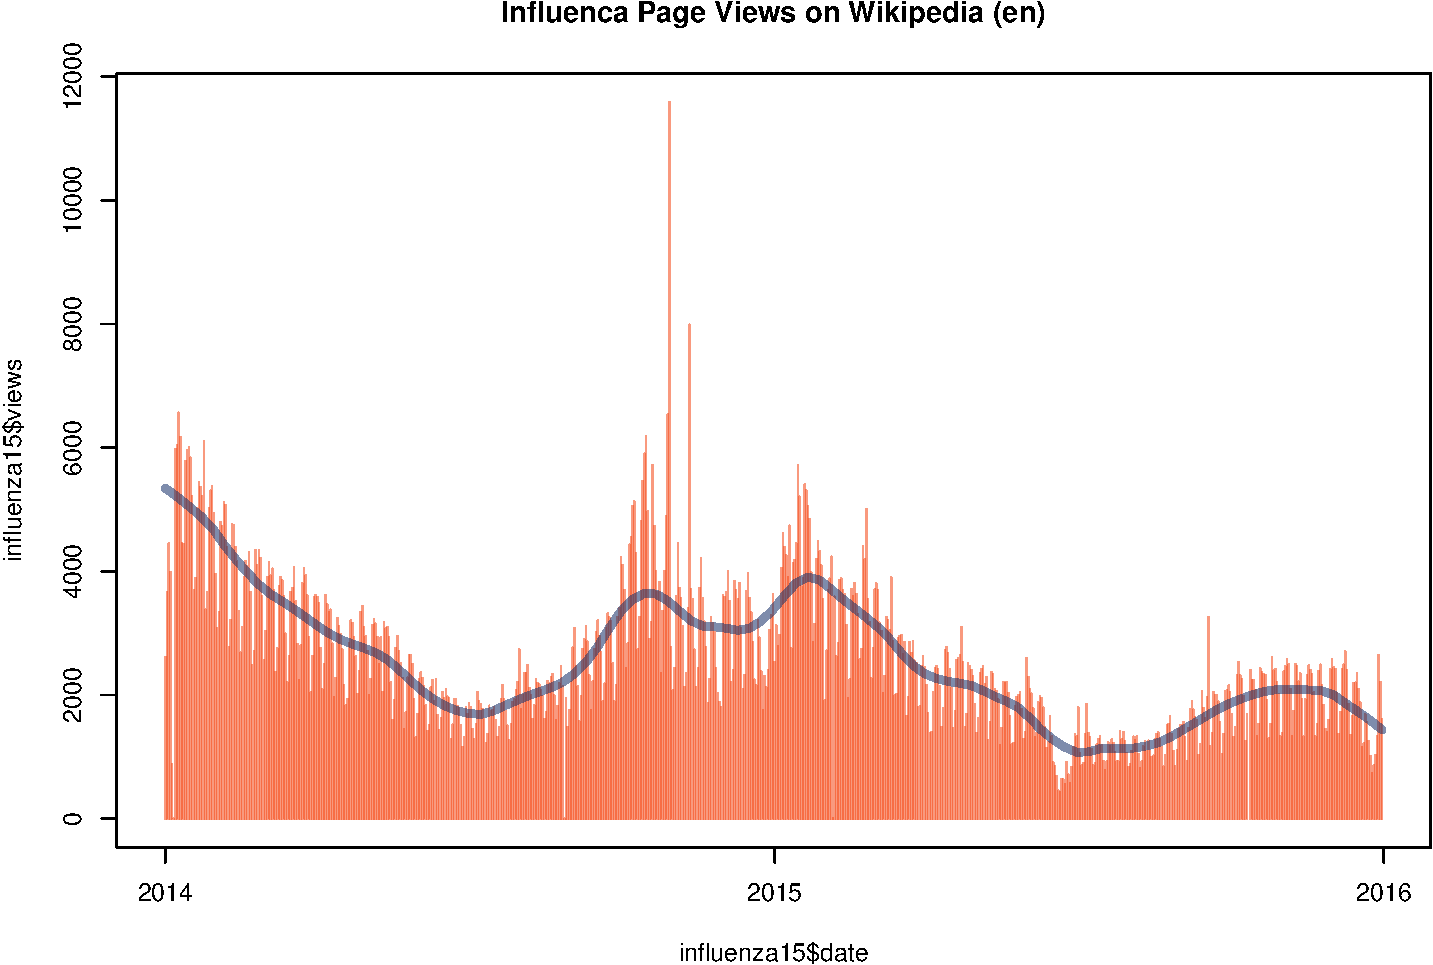
\includegraphics{json_case_files/figure-beamer/unnamed-chunk-12-1.pdf}

\end{frame}

\end{document}
